\documentclass{standalone}
\usepackage{tikz}
\usetikzlibrary{patterns, positioning}
\usepackage[sfdefault]{ClearSans} %% option 'sfdefault' activates Clear Sans as the default text font
\usepackage[T1]{fontenc}

\begin{document}
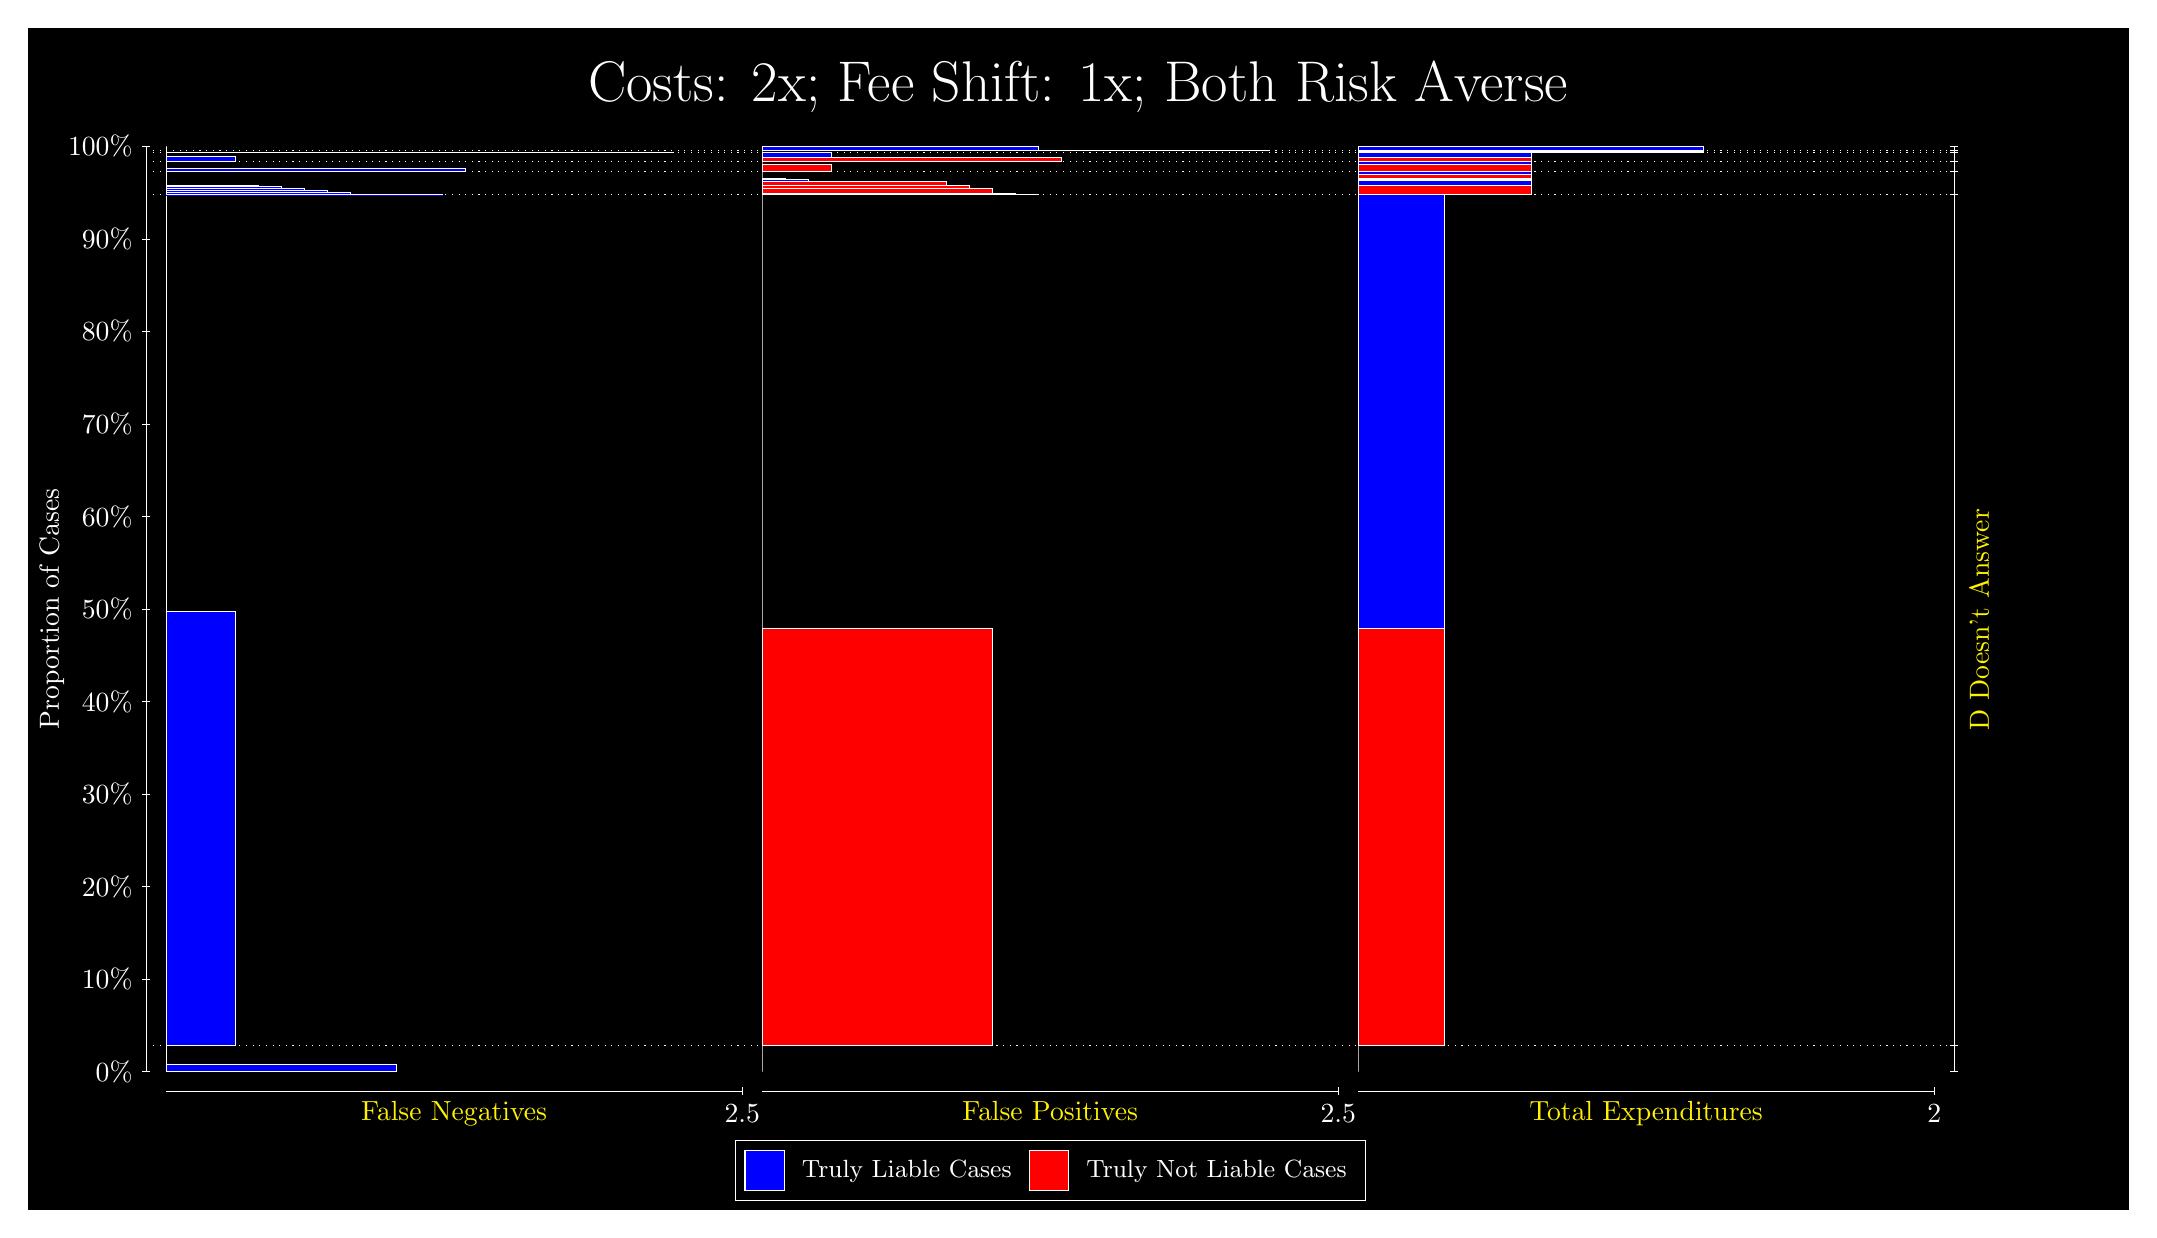
\begin{tikzpicture}
\draw[fill=black] (0,0) rectangle (26.667,15);
\draw[text=white] (0,13.5) rectangle (26.667,15) node[midway] {\huge Costs: 2x; Fee Shift: 1x; Both Risk Averse};
\draw[white, very thin] (1.5,1.75) -- (1.5,13.5);
\node[rotate=90, text=white, anchor=center] at (0.3, 7.625) {Proportion of Cases};
\draw[white, very thin] (1.45,1.75) -- (1.55,1.75);
\node[text=white, anchor=east] at (1.45, 1.75) {0\%};
\draw[white, very thin] (1.45,2.925) -- (1.55,2.925);
\node[text=white, anchor=east] at (1.45, 2.925) {10\%};
\draw[white, very thin] (1.45,4.1) -- (1.55,4.1);
\node[text=white, anchor=east] at (1.45, 4.1) {20\%};
\draw[white, very thin] (1.45,5.275) -- (1.55,5.275);
\node[text=white, anchor=east] at (1.45, 5.275) {30\%};
\draw[white, very thin] (1.45,6.45) -- (1.55,6.45);
\node[text=white, anchor=east] at (1.45, 6.45) {40\%};
\draw[white, very thin] (1.45,7.625) -- (1.55,7.625);
\node[text=white, anchor=east] at (1.45, 7.625) {50\%};
\draw[white, very thin] (1.45,8.8) -- (1.55,8.8);
\node[text=white, anchor=east] at (1.45, 8.8) {60\%};
\draw[white, very thin] (1.45,9.975) -- (1.55,9.975);
\node[text=white, anchor=east] at (1.45, 9.975) {70\%};
\draw[white, very thin] (1.45,11.15) -- (1.55,11.15);
\node[text=white, anchor=east] at (1.45, 11.15) {80\%};
\draw[white, very thin] (1.45,12.325) -- (1.55,12.325);
\node[text=white, anchor=east] at (1.45, 12.325) {90\%};
\draw[white, very thin] (1.45,13.5) -- (1.55,13.5);
\node[text=white, anchor=east] at (1.45, 13.5) {100\%};

\draw[white, very thin] (24.457,1.75) -- (24.457,13.5);
\draw[white, very thin] (24.407,1.75) -- (24.507,1.75);
\node[anchor=west] at (24.407, 1.75) {};
\draw[white, very thin] (24.407,2.0835) -- (24.507,2.0835);
\node[anchor=west] at (24.407, 2.0835) {};
\draw[white, very thin] (24.407,12.886) -- (24.507,12.886);
\node[anchor=west] at (24.407, 12.886) {};
\draw[white, very thin] (24.407,13.181) -- (24.507,13.181);
\node[anchor=west] at (24.407, 13.181) {};
\draw[white, very thin] (24.407,13.307) -- (24.507,13.307);
\node[anchor=west] at (24.407, 13.307) {};
\draw[white, very thin] (24.407,13.421) -- (24.507,13.421);
\node[anchor=west] at (24.407, 13.421) {};
\draw[white, very thin] (24.407,13.447) -- (24.507,13.447);
\node[anchor=west] at (24.407, 13.447) {};
\draw[white, very thin] (24.407,13.5) -- (24.507,13.5);
\node[anchor=west] at (24.407, 13.5) {};

\draw[white, very thin, fill=blue] (1.75,1.75) rectangle (4.6775,1.8443);
\draw[white, very thin, fill=red] (1.75,1.8443) rectangle (1.75,2.0835);
\draw[white, very thin, fill=blue] (1.75,2.0835) rectangle (2.6283,7.5923);
\draw[white, very thin, fill=red] (1.75,7.5923) rectangle (1.75,12.886);
\draw[white, very thin, fill=blue] (1.75,12.886) rectangle (5.2631,12.888);
\draw[white, very thin, fill=blue] (1.75,12.888) rectangle (4.9703,12.89);
\draw[white, very thin, fill=blue] (1.75,12.89) rectangle (4.6775,12.893);
\draw[white, very thin, fill=blue] (1.75,12.893) rectangle (4.3848,12.895);
\draw[white, very thin, fill=blue] (1.75,12.895) rectangle (4.3848,12.896);
\draw[white, very thin, fill=blue] (1.75,12.896) rectangle (4.092,12.917);
\draw[white, very thin, fill=blue] (1.75,12.917) rectangle (3.7993,12.936);
\draw[white, very thin, fill=blue] (1.75,12.936) rectangle (3.5065,12.973);
\draw[white, very thin, fill=blue] (1.75,12.973) rectangle (3.2138,12.991);
\draw[white, very thin, fill=blue] (1.75,12.991) rectangle (2.921,13.005);
\draw[white, very thin, fill=red] (1.75,13.005) rectangle (1.75,13.181);
\draw[white, very thin, fill=blue] (1.75,13.181) rectangle (5.5558,13.219);
\draw[white, very thin, fill=red] (1.75,13.219) rectangle (1.75,13.307);
\draw[white, very thin, fill=blue] (1.75,13.307) rectangle (2.6283,13.37);
\draw[white, very thin, fill=red] (1.75,13.37) rectangle (1.75,13.421);
\draw[white, very thin, fill=blue] (1.75,13.421) rectangle (8.1906,13.429);
\draw[white, very thin, fill=red] (1.75,13.429) rectangle (1.75,13.447);
\draw[white, very thin, fill=red] (1.75,13.447) rectangle (1.75,13.456);
\draw[white, very thin, fill=blue] (1.75,13.456) rectangle (1.75,13.5);
\draw[white, very thin, fill=red] (9.3189,1.75) rectangle (9.3189,1.9892);
\draw[white, very thin, fill=blue] (9.3189,1.9892) rectangle (9.3189,2.0835);
\draw[white, very thin, fill=red] (9.3189,2.0835) rectangle (12.246,7.3771);
\draw[white, very thin, fill=blue] (9.3189,7.3771) rectangle (9.3189,12.886);
\draw[white, very thin, fill=red] (9.3189,12.886) rectangle (12.832,12.893);
\draw[white, very thin, fill=red] (9.3189,12.893) rectangle (12.539,12.906);
\draw[white, very thin, fill=red] (9.3189,12.906) rectangle (12.246,12.961);
\draw[white, very thin, fill=red] (9.3189,12.961) rectangle (11.954,13.006);
\draw[white, very thin, fill=red] (9.3189,13.006) rectangle (11.661,13.052);
\draw[white, very thin, fill=red] (9.3189,13.052) rectangle (11.368,13.056);
\draw[white, very thin, fill=red] (9.3189,13.056) rectangle (11.075,13.059);
\draw[white, very thin, fill=red] (9.3189,13.059) rectangle (10.783,13.06);
\draw[white, very thin, fill=red] (9.3189,13.06) rectangle (10.49,13.062);
\draw[white, very thin, fill=blue] (9.3189,13.062) rectangle (9.9044,13.076);
\draw[white, very thin, fill=blue] (9.3189,13.076) rectangle (9.6116,13.094);
\draw[white, very thin, fill=blue] (9.3189,13.094) rectangle (9.3189,13.181);
\draw[white, very thin, fill=red] (9.3189,13.181) rectangle (10.197,13.269);
\draw[white, very thin, fill=blue] (9.3189,13.269) rectangle (9.3189,13.307);
\draw[white, very thin, fill=red] (9.3189,13.307) rectangle (13.125,13.358);
\draw[white, very thin, fill=blue] (9.3189,13.358) rectangle (10.197,13.421);
\draw[white, very thin, fill=red] (9.3189,13.421) rectangle (9.3189,13.439);
\draw[white, very thin, fill=blue] (9.3189,13.439) rectangle (9.3189,13.447);
\draw[white, very thin, fill=red] (9.3189,13.447) rectangle (15.759,13.456);
\draw[white, very thin, fill=blue] (9.3189,13.456) rectangle (12.832,13.5);
\draw[white, very thin, fill=red] (16.888,1.75) rectangle (16.888,1.9892);
\draw[white, very thin, fill=blue] (16.888,1.9892) rectangle (16.888,2.0835);
\draw[white, very thin, fill=red] (16.888,2.0835) rectangle (17.986,7.3771);
\draw[white, very thin, fill=blue] (16.888,7.3771) rectangle (17.986,12.886);
\draw[white, very thin, fill=red] (16.888,12.886) rectangle (19.083,13);
\draw[white, very thin, fill=blue] (16.888,13) rectangle (19.083,13.075);
\draw[white, very thin, fill=red] (16.888,13.075) rectangle (19.083,13.084);
\draw[white, very thin, fill=blue] (16.888,13.084) rectangle (19.083,13.093);
\draw[white, very thin, fill=red] (16.888,13.093) rectangle (19.083,13.147);
\draw[white, very thin, fill=blue] (16.888,13.147) rectangle (19.083,13.181);
\draw[white, very thin, fill=red] (16.888,13.181) rectangle (19.083,13.269);
\draw[white, very thin, fill=blue] (16.888,13.269) rectangle (19.083,13.307);
\draw[white, very thin, fill=red] (16.888,13.307) rectangle (19.083,13.358);
\draw[white, very thin, fill=blue] (16.888,13.358) rectangle (19.083,13.421);
\draw[white, very thin, fill=red] (16.888,13.421) rectangle (21.279,13.439);
\draw[white, very thin, fill=blue] (16.888,13.439) rectangle (21.279,13.447);
\draw[white, very thin, fill=red] (16.888,13.447) rectangle (21.279,13.456);
\draw[white, very thin, fill=blue] (16.888,13.456) rectangle (21.279,13.5);
\draw[white, dotted] (1.5,2.0835) -- (24.457,2.0835);
\draw[white, dotted] (1.5,12.886) -- (24.457,12.886);
\draw[white, dotted] (1.5,13.181) -- (24.457,13.181);
\draw[white, dotted] (1.5,13.307) -- (24.457,13.307);
\draw[white, dotted] (1.5,13.421) -- (24.457,13.421);
\draw[white, dotted] (1.5,13.447) -- (24.457,13.447);
\draw[white, very thin] (1.75,1.5) -- (9.0689,1.5);
\node[text=yellow, anchor=north] at (5.4094, 1.5) {False Negatives};
\draw[white, very thin] (9.0689,1.45) -- (9.0689,1.55);
\node[text=white, anchor=north] at (9.0689, 1.45) {2.5};

\draw[white, very thin] (9.3189,1.5) -- (16.638,1.5);
\node[text=yellow, anchor=north] at (12.978, 1.5) {False Positives};
\draw[white, very thin] (16.638,1.45) -- (16.638,1.55);
\node[text=white, anchor=north] at (16.638, 1.45) {2.5};

\draw[white, very thin] (16.888,1.5) -- (24.207,1.5);
\node[text=yellow, anchor=north] at (20.547, 1.5) {Total Expenditures};
\draw[white, very thin] (24.207,1.45) -- (24.207,1.55);
\node[text=white, anchor=north] at (24.207, 1.45) {2};


\node[text=yellow, centered, rotate=90] at (24.777, 7.4847) {D Doesn't Answer};






\draw (12.978300999999998,1.5) node[draw=none] (baseCoordinate) {};
\begin{scope}[align=center]
        \matrix[scale=0.5, draw=white, below=0.5cm of baseCoordinate, nodes={draw}, column sep=0.1cm]{
            \node[rectangle, draw, minimum width=0.5cm, minimum height=0.5cm, fill=blue] {}; &
            \node[draw=none, font=\small, text=white] (B) {Truly Liable Cases}; &
            \node[rectangle, draw, minimum width=0.5cm, minimum height=0.5cm, fill=red] {}; &
            \node[draw=none, font=\small, text=white] (B) {Truly Not Liable Cases}; \\
            };
\end{scope}

\end{tikzpicture}
\end{document}